\section{The Online Alignment Framework}
\label{sec:OnlineAlignmentFramework}

\subsection{Dataflow in Run II}
\label{subsec:Dataflow}
The \lhcb trigger strategies for the Run I and Run II data taking periods are shown in Figure \ref{fig:dataflow}.\\
In Run I the online event reconstruction was simpler and faster than the reconstruction used offline and did not include any information about the particle identification (PID). In order to have the same reconstruction online and offline as well as using the PID information in the \hlttwo the data-taking strategy has been amended for Run II. As in Run I a rate of 1\mhz of events passes the level-0 trigger (\lone) and is passed on to the first high level trigger stage (\hltone). There the events are partially reconstructed and accepted events are written to disk. At this stage the different alignments are run on a dedicated part of the buffered data. In case of a big shift in alignment constants the new constants are propagated to the \lhcb conditions database and used in the subsequent processing of the events by the second high level trigger (\hlttwo).\\
The alignment tasks being performed on the data are - in the order they are being run - \velo alignment, tracker alignment, \rich alignment and finally muon chamber alignment. Each alignment has its own dedicated \hltone line which collects a given number of events at the beginning of each fill (see Section \ref{subsec:HltForRich} for the \rich lines). It has been found that $\sim$1 \m events for \richone and $\sim$2\m events for \richtwo is sufficient to produce stable results. Once enough events have been collected the alignment is started.\\
\begin{figure}[htbp]
  \vspace{-0.1\baselineskip}
  \centering
  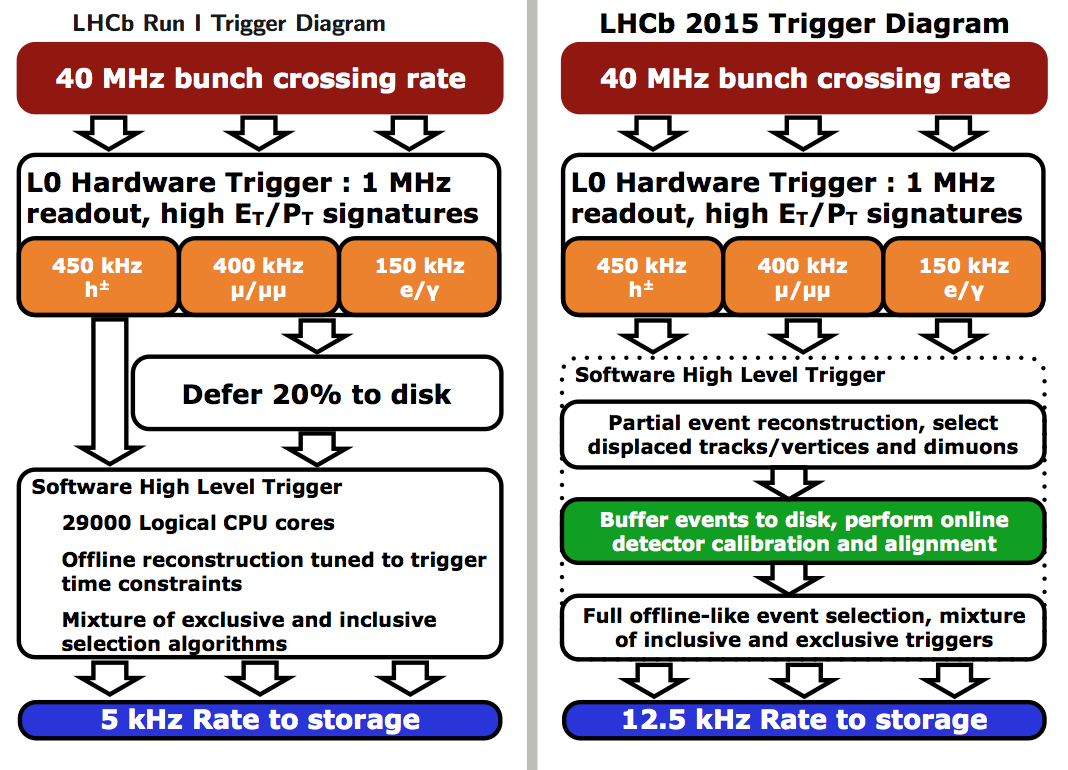
\includegraphics[width=0.75\textwidth]{figs/Online/dataflow}
  \vspace{-0.5\baselineskip}
  \caption{\lhcb dataflow for Run I (left) and Run II (right). In Run II the data is buffered after \hltone and an alignment is performed for each fill. The \hlttwo will then process the buffered events with the updated alignment constants.}
  \label{fig:dataflow}
  \vspace{-0.5\baselineskip}
\end{figure}


\subsection{\hltone selection for the \rich mirror alignment}
\label{subsec:HltForRich}
In order to determine the misalignments on the detector plane and subsequently the individual mirror misalignments the \deltatheta vs. $\phi$ histograms for each mirror combination have to contain enough entries for the fits described in Section \ref{subsec:Fitting} to converge. The minimum condition for a successful fit has been found to be that 16 of the 20 bins in $\phi$ have to contain at least 300 entries.\\
This is accomplished by having two dedicated \hltone selections, one each for \richone and \richtwo. The lines trigger on high energy particle tracks whose Cherenkov photons would populate the mirror combinations containing the fewest photons. The other mirror combinations are then populated by the rest of the tracks in the events.\\
The variables used in the selection are the track momentum $p$, the transverse track momentum $p_T$, the pseudorapidity $\eta$, the goodness of fit for the track $\chi^2$ and the polar angle of the track $\phi$. The selection criteria of tracks that are triggered upon are listed in Table \ref{tab:HltCuts}. \\

\begin{table}[htb]
  \vspace{-0.5\baselineskip}
  \caption{Trigger criteria for the \hltone line for \richone and \richtwo. Events that are accepted by these trigger lines need to have at least one track that satisfies the cuts listed below.}
  \vspace{-0.5\baselineskip}
  \centering
  \begin{tabular}{l|c|c}
  & \richone & \richtwo \\
  \hline
  momentum $p$ & $p>20$ \gev & $p>40$ \gev \\
  \hline
  transverse momentum $p_T$ & $p_T > 0.5$ \gev & $p_T > 0.5$ \gev \\
  \hline
  pseudorapidity $\eta$ & $1.6< \eta <2.04$ & $ 2.65 <\eta < 2.80 $\\
  \hline
  track $\chi^2$ & $\chi^2 < 2$ & $\chi^2 < 2$ \\
  \hline
  polar angle $\Phi$ & $-2.65< \Phi <-2.30$ & $-2.59< \Phi <-2.49$ \\
   & $-0.80 < \Phi <-0.50 $ & $-0.65 < \Phi <-0.55 $ \\
   & $0.50 < \Phi < 0.80$ & $ 0.55 < \Phi < 0.65 $ \\
   &  $ 2.30 < \Phi <2.65 $ & $2.49 < \Phi < 2.59 $ \\
  \end{tabular}
  \label{tab:HltCuts}
  \vspace{-0.5\baselineskip}
\end{table}

\subsection{The Alignment Farm}
\label{subsec:AlignmentFarm}
All alignments are run on the alignment farm. The alignment farm consists of approximately 1700 CPUs, called \textit{analysers} and a central node called the \textit{iterator}.\\
The data taken from the \hltone selection for the \rich alignments is stored evenly distributed over the analysers until it can be processed by \hlttwo. The analysers perform the event reconstruction with a database provided to them by the iterator and fill the \deltatheta vs. $\phi$ histograms mentioned in Section \ref{sec:MirrorAlignmentMethod}. Apart from providing the database with the desired mirror orientations the iterator also performs the fits on the histograms, determines the individual mirror misalignments, produces a new database and decides whether the alignment procedure has converged or whether another iteration has to be performed. If the latter is the case, the iterator will make the new database available to the analysers (for more details see Section \ref{subsec:implementation}).\\
The advantage of having a system consisting of about 1700 nodes distributed over 50 farms is that the event reconstruction can happen in parallel and is therefore very fast. This parallel processing is asynchronous and has to be coordinated between the individual analysers and the iterator which is described in the next section.\\


\subsection{The Control Flow}
The execution of the alignment tasks is under the control of the LHCb Experiment Control System (ECS), and is implemented as a \textit{finite state machine}, which is illustrated in Figure \ref{fig:states}. The principle of a finite state machine means that each component of the system (here every individual analyser and the iterator) has to be in one of a finite number of states at all times. The states used for the alignment procedure are also shown in Figure \ref{fig:states}, such as ``READY'', ``RUNNING'' and ``PAUSED''. The alignment is then steered by the \textit{run control} that can see all the components and their individual states and can send commands. Those commands will be received by the individual components and they will act accordingly. For a given state only a certain number of commands are possible - for example if the component is in state ``PAUSED'' it can only receive the commands ``continue'' and ``stop''. If a command is received the component will go from its state into the state declared by Figure \ref{fig:states}. When in a new state the component will usually perform a task and then set itself into another state once finished so that the run control is aware of this task being completed.\\ 

\begin{figure}[htbp]
  \vspace{-0.5\baselineskip}
  \centering
  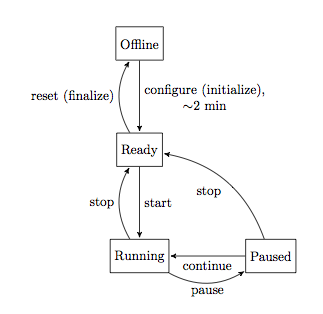
\includegraphics[width=0.7\textwidth]{figs/Online/states}
  \vspace{-0.5\baselineskip}
  \caption{Example of one component within a system functioning under the principle of a finite state machine. The boxes show the states the component is in while the arrows show the commands the component gets from the run control.}
  \label{fig:states}
  \vspace{-0.5\baselineskip}
\end{figure}


\subsection{Implementation of the \rich Mirror Alignment for Run II}
\label{subsec:implementation}
The interplay between the iterator, one example analyser and the run control during the course of the alignment of a \rich detector is shown in Figure \ref{fig:runcontrol}.\\
The individual analysers and the iterator all follow the same sequence of states, namely the one shown in Figure \ref{fig:states}. When the alignment is being started the run control sends the command to ``configure'' to both the iterator and all analysers. All components will go into state ``CONFIGURING'' while setting up to run the alignment. For the analysers this means that they read in the configuration for the reconstruction of the events, while the iterator sets up a directory in which all files for this alignment are saved.\\
Each component goes into state ``READY'' when it is done configuring. When all tasks are in the ``READY'' state, the iterator makes an initial set of alignment constants available to the analysers and then updates its state to ``RUNNING''. The analyzers are then sent the``start'' command, update their state to ``RUNNING'' and start reconstructing the data stored on them. Each analyser that has completed processing its data updates its state to ``PAUSED'', and once they have all reached this state, the run control sends the “stop” command and they update their states to ``READY''. The iterator is then sent the ``pause'' command, collects and combines the histograms produced by the analyser tasks and performs the fits. It then calculates the individual mirror misalignments and produces a new database containing the mirror orientations. The it either indicates that conversion has been reached by updating its state to ``READY'', or that further iteration is required by updating its state ``RUNNING''. In the latter case the iterator will provide the new database to the analysers before changing its state and another iteration is started.\\

\begin{figure}[htbp]
  \vspace{-0.5\baselineskip}
  \centering
  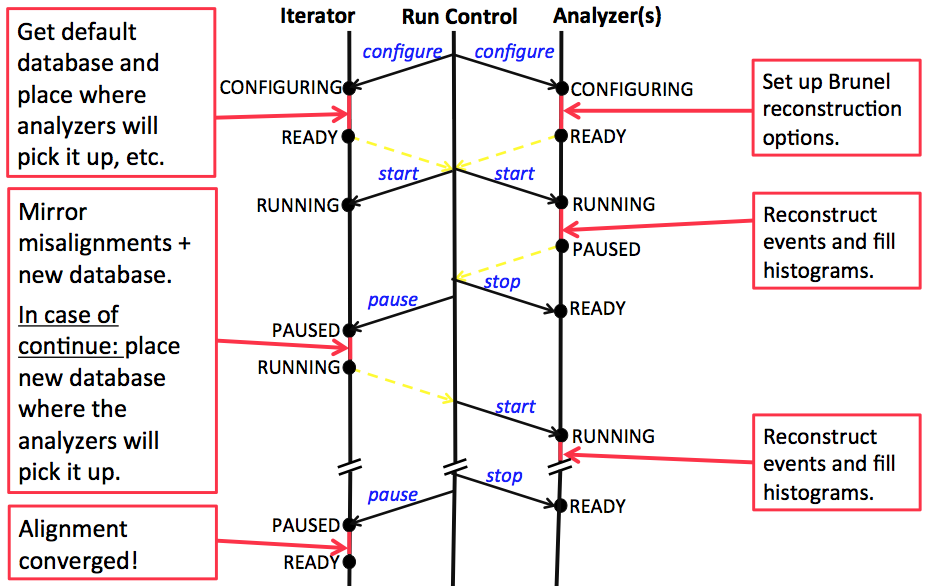
\includegraphics[width=\textwidth]{figs/Online/runcontrol}
  \vspace{-0.5\baselineskip}
  \caption{Interplay between the iterator, one example analyser and the run control during the \rich alignment procedure. The analysers reconstruct the data and produce the histograms that the iterator evaluates. The run control makes sends commands to the iterator and the analysers to make sure the alignment procedure happens in the necessary sequence. }
  \label{fig:runcontrol}
  \vspace{-0.5\baselineskip}
\end{figure}